\documentclass[11pt]{beamer}
\usetheme{CambridgeUS}
%\usecolortheme{orchid}

% Packages
\usepackage[utf8]{inputenc}
\usepackage{lmodern}
\usepackage{amsmath}
\usepackage{amsfonts}
\usepackage{amssymb}
\usepackage{graphicx}
\usepackage{svg}
\usepackage{wasysym}
\usepackage{hyperref}

% Headers
\author[Fassina, Ranzato, Zanella]{Nicolò Fassina, Francesco Ranzato, Marco Zanella}
\title[Robustness of kNN]{Robustness Certification of k-Nearest Neighbors}

% Options
\setbeamercovered{transparent}
\setbeamertemplate{navigation symbols}{} 
\logo{
\includegraphics[width=0.5cm]{assets/logo/unipd}}
\institute[Univ. Padova]{University of Padova}
\date{December 4, 2023}
%\subject{}
\DeclareTextFontCommand{\emph}{\bfseries}

% Document
\begin{document}

\begin{frame}
\titlepage
\end{frame}

\begin{frame}{Outline}
\tableofcontents
\end{frame}

\section{Introduction}
\begin{frame}{Introduction $>$ kNN}
\emph{k-nearest neighbors}: suitable for \emph{classification} and regression

\begin{center}
 \includesvg[width=0.9\textwidth]{assets/figures/knn}
\end{center}

Relies on \emph{distance metrics}: Manhattan $\mu$, Euclidean $\eta$, Minkowski $\delta_p$ \ldots
\end{frame}

\begin{frame}{Introduction $>$ Stability}
\emph{Stablity} (around a point)

\begin{center}
 \includesvg[width=0.9\textwidth]{assets/figures/stability-1}
\end{center}

Output is not influenced by \emph{small alterations}
\end{frame}

\begin{frame}{Introduction $>$ Stability}
\emph{Geometric} view of a classifier

\begin{center}
 \includesvg[width=0.9\textwidth]{assets/figures/stability-2}
\end{center}

Similar samples, \emph{different classification}
\end{frame}

\begin{frame}{Introduction $>$ Abstract Interpretation}
\emph{Abstract Interpretation}: forget details, focus on \emph{properties of interest}

\vspace{2em}

\emph{Collecting semantics}: sets of points instead of single points
\begin{center}
 $C(1) = \bigstar$ \hspace{1.5em}
 $C(3) = \bigstar$ \hspace{1.5em} 
 $C(4) = \leftmoon$ \hspace{1.5em}
 $C(6) = \bigstar$
\end{center}

\begin{center}
 $C(\{1, 3, 4, 6\}) = \{\bigstar, \leftmoon\}$
\end{center}

\begin{center}
 $C^A([1, 6]) = \{\bigstar, \leftmoon\}$
\end{center}
Single \emph{abstract value} to represent (possibly infinite) sets
\end{frame}

\begin{frame}{Introduction $>$ Abstract Interpretation}
Abstract Interpretation guarantees \emph{soundness}

\begin{center}
$C(\{1, 3, 4, 6\}) = \{\bigstar, \leftmoon\}$

\vspace{1.5em}

\begin{tabular}{c c c}
 $C^A([1, 6]) = \{\bigstar\}$ &
 $C^A([1, 6]) = \{\bigstar, \leftmoon, \bigcirc\}$ &
 $C^A([1, 6]) = \{\bigstar, \leftmoon\}$ \\
 unsound & sound & complete
\end{tabular}
\end{center}

\emph{Formally}
\begin{center}
$X \subseteq \gamma^A(a) \Rightarrow C(X) \subseteq \gamma^A(C^A(a))$
\end{center}

\emph{Less formally}
\begin{center}
if $C^A(X^A) = \{l\}$, then $C$ is \emph{stable} over $X$

$C^A(X^A)$ is a \emph{superset} of the labels of $C(X)$
\end{center}
\end{frame}

\begin{frame}{Introduction $>$ Abstract Interpretation}
\emph{Abstract domain}: properties to focus on
\vspace{0.5em}
\begin{columns}
 \begin{column}{0.32\textwidth}
  \centering
  \emph{interval}
  
  \includesvg[width=0.6\textwidth]{assets/figures/abstract-interpretation-domain-1}
  
  fast
 \end{column}
 
 \begin{column}{0.32\textwidth}
  \centering
  \emph{octagon}
  
  \includesvg[width=0.6\textwidth]{assets/figures/abstract-interpretation-domain-2}
  
  relational
 \end{column}
 
 \begin{column}{0.32\textwidth}
  \centering
  \emph{polyhedron}
  
  \includesvg[width=0.6\textwidth]{assets/figures/abstract-interpretation-domain-3}
  
  expensive
 \end{column}
\end{columns}
\vspace{1em}

\emph{Interval-like} abstractions
\vspace{0.5em}
\begin{columns}
 \begin{column}{0.32\textwidth}
  \centering
  \emph{interval}
  
  \vspace{0.5em}
  \includesvg[width=0.75\textwidth]{assets/figures/abstract-interpretation-example-1}
  
  $[l, h]$
 \end{column}
 
 \begin{column}{0.32\textwidth}
  \centering
  \emph{RAF}
  
  \vspace{0.5em}
  \includesvg[width=0.75\textwidth]{assets/figures/abstract-interpretation-example-2}
  
  $c + a\epsilon_1 + b\epsilon_2 + z\epsilon_r$
 \end{column}
 
 \begin{column}{0.32\textwidth}
  \centering
  \emph{zonotope}
  
  \vspace{0.5em}
  \includesvg[width=0.75\textwidth]{assets/figures/abstract-interpretation-example-3}
  
  $c + a\epsilon_1 + b\epsilon_2 + u\epsilon_1^2 + v\epsilon_2^4$
 \end{column}
\end{columns}
\end{frame}


\section{Our Approach}
\begin{frame}{Our Approach $>$ Overview}
Analysis of one \emph{sample subject to a perturbation}:
\begin{enumerate}
 \item perturbation to \emph{abstract value}
 \item computation of \emph{abstract distances}
 \item \emph{sorting} neighbors
 \item computation of \emph{abstract scores} for labels
 \item computation of \emph{superset of labels}
 \item \emph{applications}
\end{enumerate}
\end{frame}

\begin{frame}{Our Approach $>$ Perturbation and Abstract Input}
Given
\begin{center}
 $x \in \mathbb{R}^n$
 \hspace{2em}
 $P: \mathbb{R}^n \rightarrow \wp(\mathbb{R}^n)$
 \hspace{2em} 
 $\alpha^A: \wp(\mathbb{R}^n) \rightarrow A$
\end{center}

Compute
\begin{center}
 $a = \alpha^A(P(x))$
 
 \includesvg[width=0.25\textwidth]{assets/figures/abstraction-1}
 \includesvg[width=0.25\textwidth]{assets/figures/abstraction-2}
 \includesvg[width=0.25\textwidth]{assets/figures/abstraction-3}
\end{center}
 
\begin{center}
 $P(x) = \{x' \in \mathbb{R}^n ~|~ ||x - x'||_\infty < \epsilon\}$	
 $a = [[x_1 - l_1, x_1 + u_1], \ldots, [x_n - l_n, x_n + u_n]]$	
\end{center}
\end{frame}

\begin{frame}{Our Approach $>$ Abstract Distance}
Overapproximate \emph{distances} $\delta^A(a, \cdot)$ from neighbors
\begin{columns}
 \begin{column}{0.35\textwidth}
  \begin{center}
   \includesvg[width=0.95\textwidth]{assets/figures/abstract-distance}
  \end{center}
 \end{column}
 \begin{column}{0.65\textwidth}
  Manhattan distance:
  
  $\mu(x, x') = |x_1 - x'_1| + \ldots + |x_n - x'_n|$
  
  $\mu^A(a, x') = |a_1 -^A x'_1|^A +^A \ldots +^A |a_n -^A x'_n|^A$

  \vspace{1em}
  Euclidean distance:
  
  $\eta(x, x') = (x_1 - x'_1)^2 + \ldots + (x_n - x'_n)^2$
  
  $\eta^A(a, x') = (a_1 -^A x'_1)^{2^A} +^A \ldots +^A (a_n -^A x'_n)^{2^A}$
  
  \vspace{1em}
  General Minkowski distance:
  
  $\delta_p(x, x') = |x_1 - x'_1|^p + \ldots + |x_n - x'_n|^p$
  
  $\delta^A_p(a, x') = |a_1 -^A x'_1|^{p^A} +^A \ldots +^A |a_n -^A x'_n|^{p^A}$
 \end{column}
\end{columns}

\begin{center}
$\delta^A(a, \bigstar_1) = [0.3, 1.4]$
\hspace{1em}
$\delta^A(a, \leftmoon_1) = [1.7, 2.4]$
\hspace{1em}
\ldots
\end{center}
\end{frame}

\begin{frame}{Our Approach $>$ Sorting Neighbors}
Use abstract distances $\delta^A(a, \cdot)$
\begin{center}
$\bigstar_1: [0.3, 1.4]$
\hspace{1.0em}
$\bigstar_2: [1.5, 1.9]$
\hspace{1.0em}
$\leftmoon_1: [1.7, 2.4]$
\hspace{1.0em}
$\bigstar_3: [2.0, 2.7]$
\end{center}

To determine \emph{closest neighbors}:
\begin{align*}
& \bigstar_1 <^A \bigstar_2 & \bigstar_1 <^A \leftmoon_1 & \bigstar_1 <^A \bigstar_3
& \Rightarrow \bigstar_1 \text{~closest neighbor}
\\
& \bigstar_2 \not<^A \leftmoon_1 & \bigstar_2 <^A \bigstar_3 &
& \Rightarrow \bigstar_2, \leftmoon_1 \text{~2nd closest neighbor}
\\
& \leftmoon_1 \not<^A \bigstar_3 & &
&\Rightarrow \leftmoon_1, \bigstar_3 \text{~3rd closest neighbor}
\\
& \ldots & & &
\end{align*}

Three-closest neighbors $\subseteq \{\bigstar_1, \bigstar_2, \leftmoon_1, \bigstar_3\}$
\end{frame}

\begin{frame}{Our Approach $>$ Abstract Score}
\begin{center}
 $score_\bigstar = [0, 0]$
 \hspace{1.5em}
 $score_{\leftmoon} = [0, 0]$
 \hspace{1.5em}
 $score_{\bigcirc} = [0, 0]$
\end{center}

For every neighbor in $\{\bigstar_1, \bigstar_2, \leftmoon_1, \bigstar_3\}$
\begin{itemize}
 \item $\bigstar_1$ is \emph{certain}: $score_\bigstar = [1, 1]$
 \item $\bigstar_2$ \emph{may be} a neighbor: $score_\bigstar = [1, 2]$
 \item $\leftmoon_1$ \emph{may be} a neighbor: $score_{\leftmoon} = [0, 1]$
 \item $\bigstar_3$ \emph{may be} a neighbor: $score_\bigstar = [1, 3]$
\end{itemize}

\begin{center}
 $score_\bigstar = [1, 3]$
 \hspace{1.5em}
 $score_{\leftmoon} = [0, 1]$
 \hspace{1.5em}
 $score_{\bigcirc} = [0, 0]$
\end{center}

Adjust scores
\begin{center}
 $score_\bigstar = [2, 3]$
 \hspace{1.5em}
 $score_{\leftmoon} = [0, 1]$
 \hspace{1.5em}
 $score_{\bigcirc} = [0, 0]$
\end{center}
\end{frame}

\begin{frame}{Our Approach $>$ Overapproximation of Labels}
Pick \emph{dominating labels}
\begin{center}
 \includesvg[width=0.9\textwidth]{assets/figures/labels}
 
 $score_\bigstar > score_{\leftmoon}$
 \hspace{1em}
 $score_\bigstar > score_{\bigcirc}$
\end{center}

$C^A(a) = \{\bigstar\} \Rightarrow \forall x' \in P(x)\colon C(x) = \bigstar$
\hspace{2em}
$C$ is \emph{stable} over $P(x)$
\end{frame}

\begin{frame}{Our Approach $>$ Applications}
\begin{columns}
 \begin{column}{0.5\textwidth}
  \centering
  \emph{Robustness}
  
  $C$ correct on $x$ and stable over $P(x)$
  
  then $C$ \emph{robust} over $P(x)$
  
  \begin{center}
   \includesvg[width=0.9\textwidth]{assets/figures/robustness}
  \end{center}
  \[
   C(x) = y, \forall x' \in P(x)\colon C(x') = C(x)
  \]
 \end{column}
 \begin{column}{0.5\textwidth}
  \centering
  \emph{Individual Fairness}
  
  \emph{Similar} individuals treated in the \emph{same way}
  
  \begin{center}
   \includesvg[width=0.9\textwidth]{assets/figures/fairness}
  \end{center}
  \[
   \forall x' \colon \delta(x, x') < \epsilon \Rightarrow C(x) = C(x')
  \]
 \end{column}
\end{columns}
\end{frame}

\section{Results}
\begin{frame}{Results}
Our playground
\begin{center}
 \begin{tabular}{r | r r r r}
  dataset       & \# training & \# test & \# features & \# labels \\
  \hline
  australian    &         483 &     207 &          39 &         2 \\
  breast cancer &         479 &     204 &          10 &         2 \\
  diabetes      &         556 &     230 &           8 &         2 \\
  fourclass     &         604 &     258 &           2 &         2 \\
  letter        &       15000 &    5000 &          16 &        26 \\
  pendigits     &        7494 &    3498 &          16 &        10 \\
  satimage      &        4435 &    2000 &          46 &         6 \\
  \hline
  compas        &        4222 &    1056 &         370 &         2 \\
  german        &         800 &     200 &          56 &         2
 \end{tabular}
\end{center}

$\forall k \in \{1, 3, 5, 7\} \times \delta \in \{\mu, \eta\} \times a \in \{Interval, RAFs\} \times \epsilon \in [0, 0.1]$

\begin{center}
 check out NAVe at
 \url{https://github.com/abstract-machine-learning/NAVe}
\end{center}
\end{frame}

\begin{frame}{Results $>$ Effectiveness of Abstractions}
Interval vs RAF: paradigmatic example
\begin{center}
 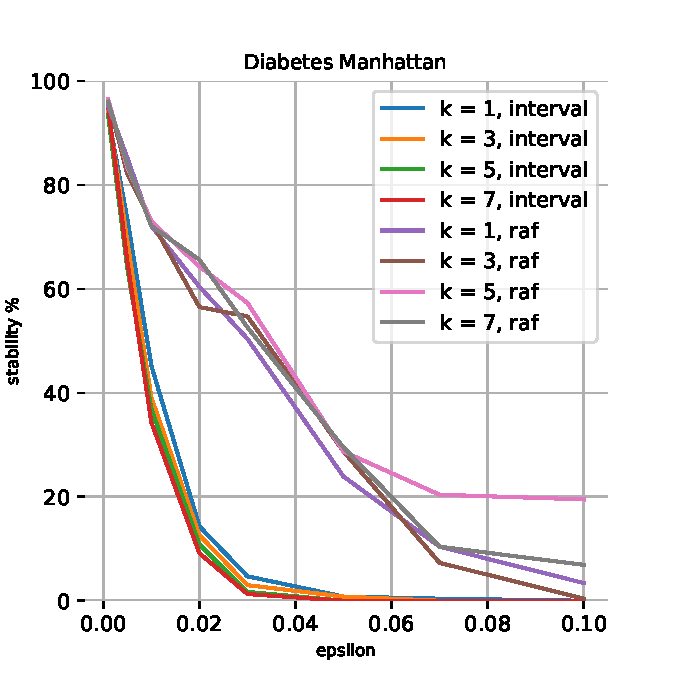
\includegraphics[width=0.49\textwidth]{assets/charts/diabetes-manhattan}
 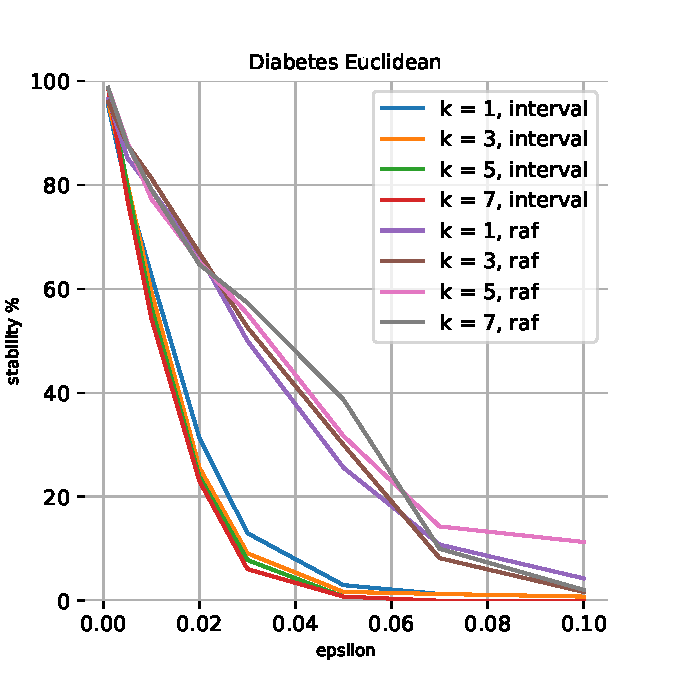
\includegraphics[width=0.49\textwidth]{assets/charts/diabetes-euclidean}
\end{center}
RAFs usually provides \emph{less false positives}
\end{frame}

\begin{frame}{Results $>$ Efficiency of Abstractions}
Average verification time per sample (s)
\begin{center}
 \begin{tabular}{r | r r | r r}
                & \multicolumn{2}{c|}{Interval} & \multicolumn{2}{c}{RAF}\\
  dataset       & $\mu$ & $\eta$ & $\mu$ & $\eta$\\
  \hline
  australian    &  0.01 &   0.01 &  0.11 &  0.22 \\  
  breast cancer &  0.01 &   0.01 &  0.06 &  0.05 \\  
  diabetes      &  0.11 &   0.07 &  0.55 &  0.58 \\  
  fourclass     &  0.04 &   0.04 &  0.35 &  0.40 \\  
  letter        &  5.44 &   4.97 & 21.89 & 22.64 \\  
  pendigits     &  0.26 &   0.57 &  9.99 &  9.70 \\  
  satimage      &  0.33 &   2.90 & 11.91 &  4.29 \\  
  \hline
  Compas        & 15.30 &  18.48 & 140.82& 239.99\\ 
  German        &  0.75 &   0.74 &  5.08&   7.67\\
 \end{tabular}
\end{center}
RAF \emph{more expensive} by one order of magnitude
\end{frame}

\begin{frame}{Results $>$ Improvements by RAF}
RAF gain: paradigmatic example
\begin{center}
 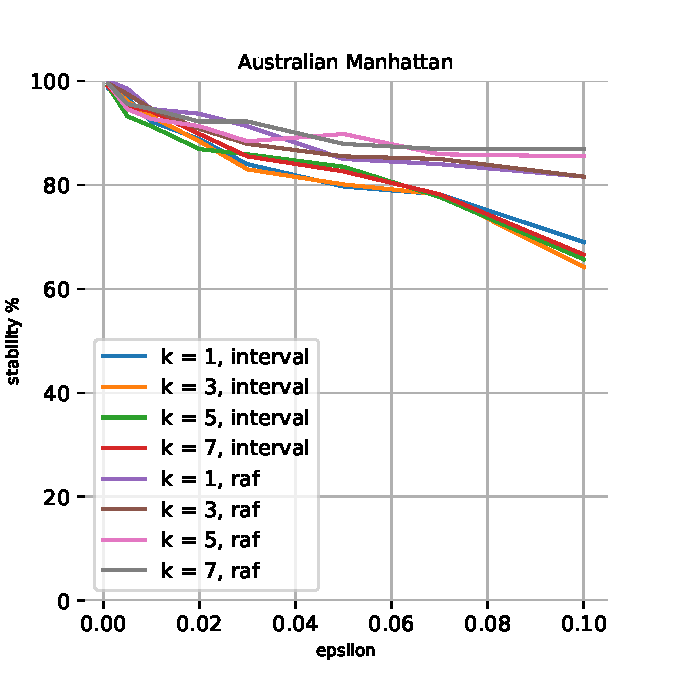
\includegraphics[width=0.49\textwidth]{assets/charts/australian-manhattan}
 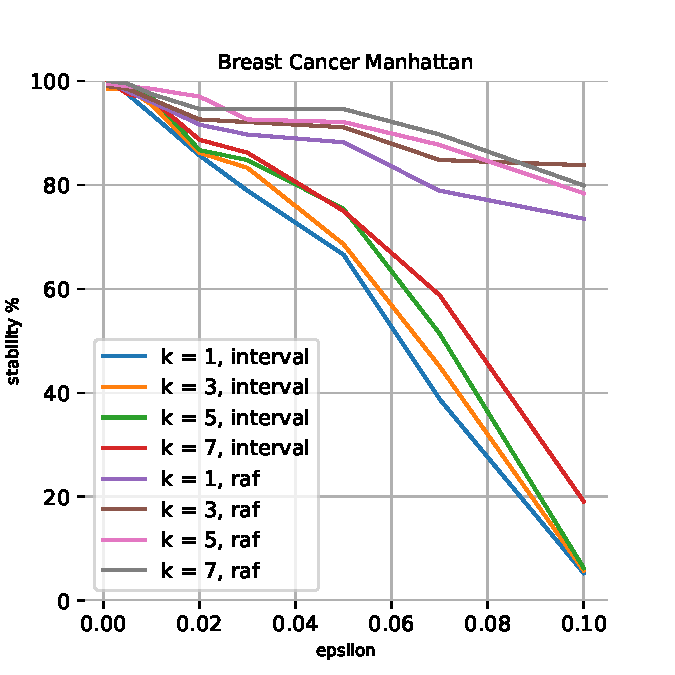
\includegraphics[width=0.49\textwidth]{assets/charts/breast-cancer-manhattan}
\end{center}
RAFs improvements \emph{domain-specific}
\end{frame}

\begin{frame}{Results $>$ Fairness}
Fairness as stability
\begin{center}
 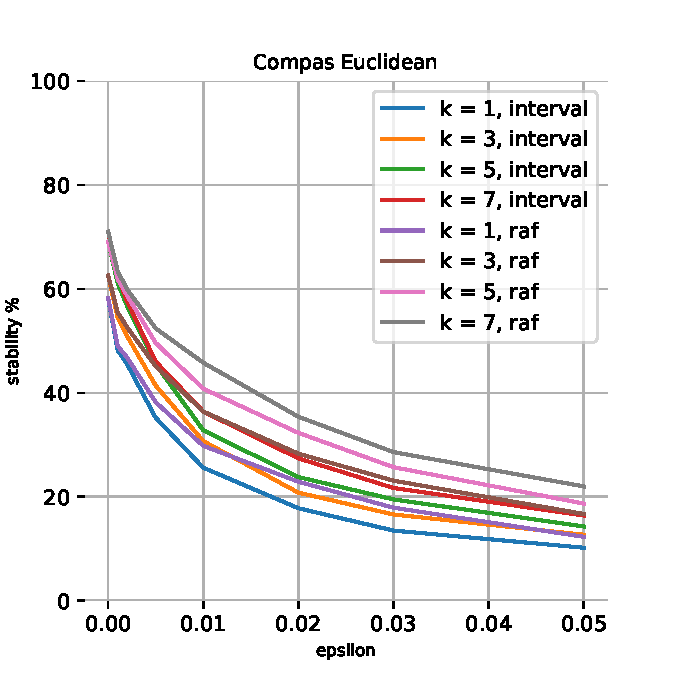
\includegraphics[width=0.49\textwidth]{assets/charts/compas-euclidean}
 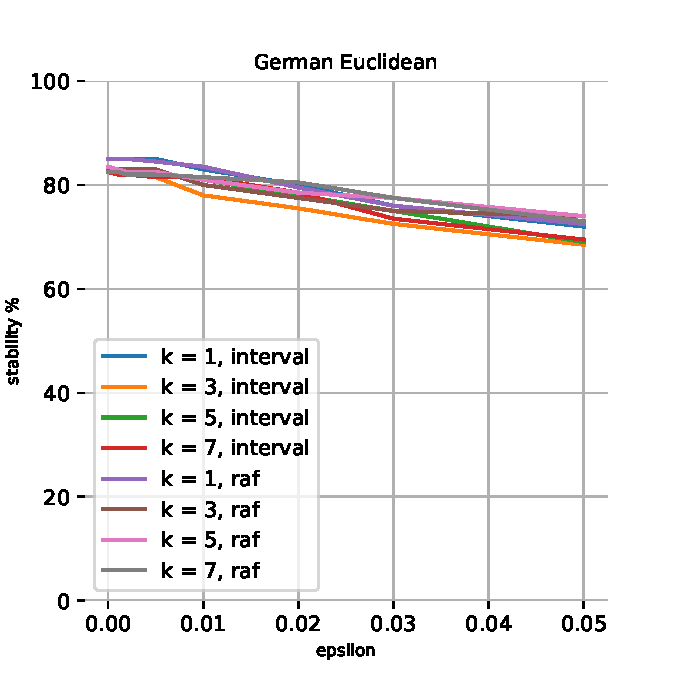
\includegraphics[width=0.49\textwidth]{assets/charts/german-euclidean}
\end{center}
Behavior mostly \emph{domain-specific}
\end{frame}

\section{Conclusion}
\begin{frame}{Conclusion}
\begin{center}
 \Large\emph{sum-up}
\end{center}

\begin{columns}
 \begin{column}{0.25\textwidth}
  \centering
  \includesvg[width=0.5\textwidth]{assets/symbols/star}\\
  backed-up by \emph{formal methods} and proofs
 \end{column}
 \begin{column}{0.25\textwidth}
  \centering
  \includesvg[width=0.5\textwidth]{assets/symbols/moon}\\
  tunable to \emph{different abstractions}
 \end{column}
 \begin{column}{0.25\textwidth}
  \centering
  \includesvg[width=0.5\textwidth]{assets/symbols/earth}\\
  good performance during \emph{experiments}
 \end{column}
 \begin{column}{0.25\textwidth}
  \centering
  \includesvg[width=0.5\textwidth]{assets/symbols/dot}\\
  room for improvement: \emph{completeness}
 \end{column}
\end{columns}

\vspace{2em}
\begin{center}
 check out NAVe at
 \url{https://github.com/abstract-machine-learning/NAVe}
\end{center}
\end{frame}

\begin{frame}{}
 \centering
 \Large
 \emph{Thank you!}
 
 \vspace{1em}
 \includesvg[width=0.9\textwidth]{assets/figures/final} 
\end{frame}

\end{document}